% Options for packages loaded elsewhere
\PassOptionsToPackage{unicode}{hyperref}
\PassOptionsToPackage{hyphens}{url}
%
\documentclass[
]{article}
\usepackage{amsmath,amssymb}
\usepackage{lmodern}
\usepackage{iftex}
\ifPDFTeX
  \usepackage[T1]{fontenc}
  \usepackage[utf8]{inputenc}
  \usepackage{textcomp} % provide euro and other symbols
\else % if luatex or xetex
  \usepackage{unicode-math}
  \defaultfontfeatures{Scale=MatchLowercase}
  \defaultfontfeatures[\rmfamily]{Ligatures=TeX,Scale=1}
\fi
% Use upquote if available, for straight quotes in verbatim environments
\IfFileExists{upquote.sty}{\usepackage{upquote}}{}
\IfFileExists{microtype.sty}{% use microtype if available
  \usepackage[]{microtype}
  \UseMicrotypeSet[protrusion]{basicmath} % disable protrusion for tt fonts
}{}
\makeatletter
\@ifundefined{KOMAClassName}{% if non-KOMA class
  \IfFileExists{parskip.sty}{%
    \usepackage{parskip}
  }{% else
    \setlength{\parindent}{0pt}
    \setlength{\parskip}{6pt plus 2pt minus 1pt}}
}{% if KOMA class
  \KOMAoptions{parskip=half}}
\makeatother
\usepackage{xcolor}
\IfFileExists{xurl.sty}{\usepackage{xurl}}{} % add URL line breaks if available
\IfFileExists{bookmark.sty}{\usepackage{bookmark}}{\usepackage{hyperref}}
\hypersetup{
  pdftitle={Multivarate Permuation Analysis},
  pdfauthor={Nutcha Wattanachit, Johannes Bracher, Evan Ray, Nick Reich},
  hidelinks,
  pdfcreator={LaTeX via pandoc}}
\urlstyle{same} % disable monospaced font for URLs
\usepackage[margin=1in]{geometry}
\usepackage{graphicx}
\makeatletter
\def\maxwidth{\ifdim\Gin@nat@width>\linewidth\linewidth\else\Gin@nat@width\fi}
\def\maxheight{\ifdim\Gin@nat@height>\textheight\textheight\else\Gin@nat@height\fi}
\makeatother
% Scale images if necessary, so that they will not overflow the page
% margins by default, and it is still possible to overwrite the defaults
% using explicit options in \includegraphics[width, height, ...]{}
\setkeys{Gin}{width=\maxwidth,height=\maxheight,keepaspectratio}
% Set default figure placement to htbp
\makeatletter
\def\fps@figure{htbp}
\makeatother
\setlength{\emergencystretch}{3em} % prevent overfull lines
\providecommand{\tightlist}{%
  \setlength{\itemsep}{0pt}\setlength{\parskip}{0pt}}
\setcounter{secnumdepth}{-\maxdimen} % remove section numbering
\usepackage{tabularx}
\usepackage{hyperref}
\usepackage{wrapfig}
\usepackage{float}
\usepackage{colortbl}
\usepackage{pdflscape}
\usepackage{tabu}
\usepackage{xcolor}
\ifLuaTeX
  \usepackage{selnolig}  % disable illegal ligatures
\fi

\title{Multivarate Permuation Analysis}
\author{Nutcha Wattanachit, Johannes Bracher, Evan Ray, Nick Reich}
\date{10/25/2022}

\begin{document}
\maketitle

\hypertarget{similarity-by-type-during-the-winter-20202021-wave}{%
\section{Similarity by type during the winter 2020/2021
wave}\label{similarity-by-type-during-the-winter-20202021-wave}}

The Delta wave in the fall? 8 weeks of increasing with not more than 2
negative growths, averaging more than 200 deaths during 2021-06-15 and
2021-11-01 period (this is location criteria). Take overall submissions
(total submission during overall during the period in the overall
analysis) into account to indicate some commitment - at 70 percents of
the max of 344 sub in each location during may 2 2020 and 2021 dec 18 -
excluding baseline model.

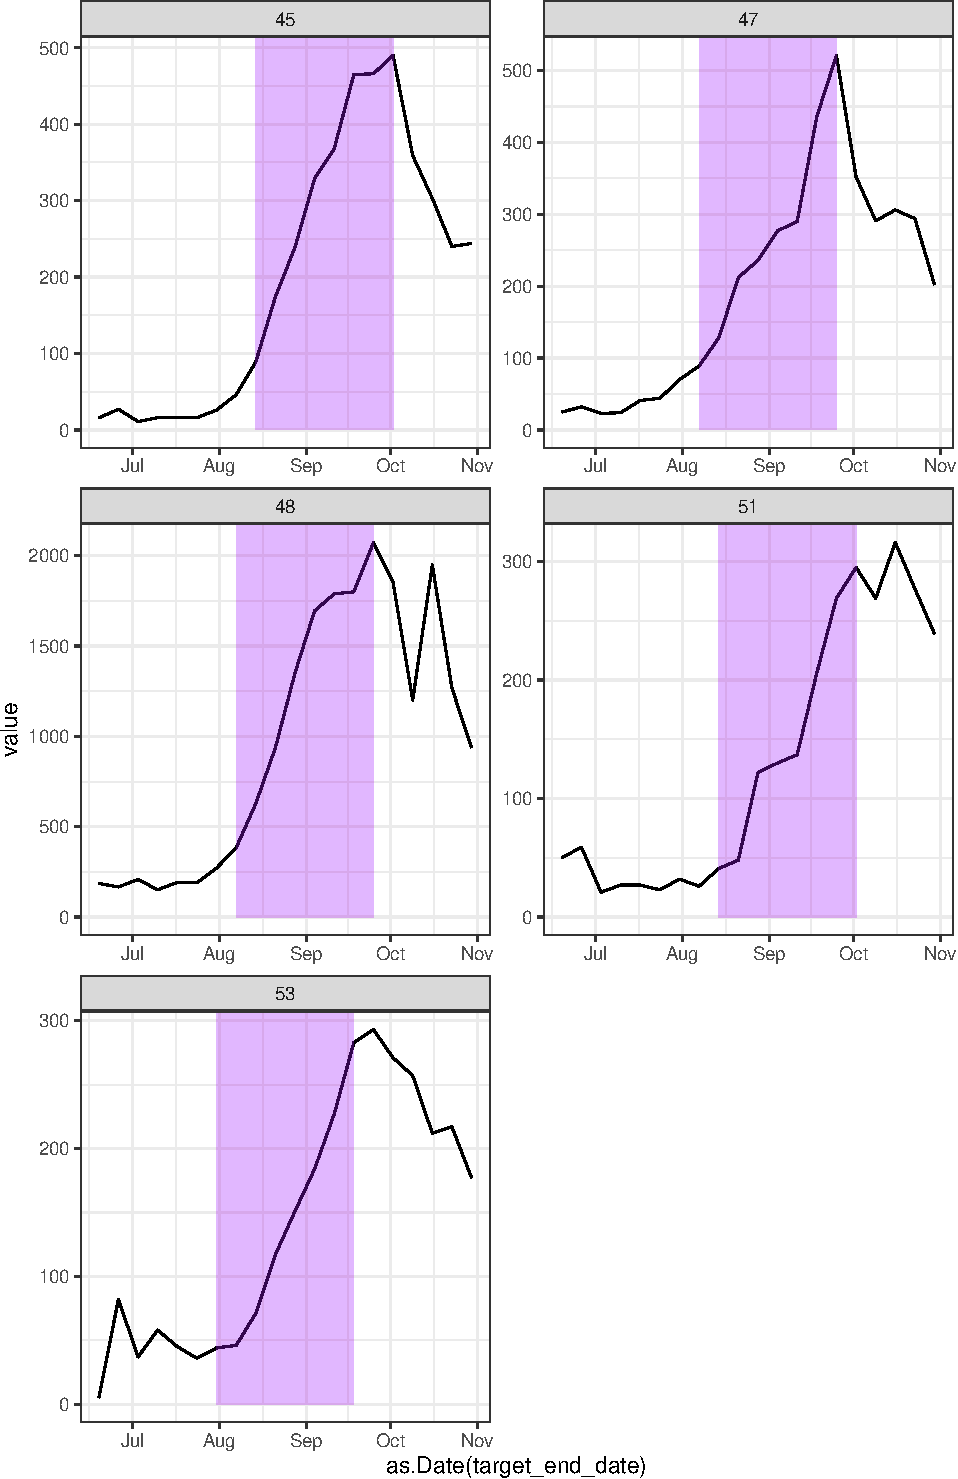
\includegraphics{multi_perm_analysis_files/figure-latex/p1-1.pdf}

\hypertarget{boxplots-of-approx.-cds-by-categories}{%
\subsection{Boxplots of approx. CDs by
categories}\label{boxplots-of-approx.-cds-by-categories}}

\begin{center}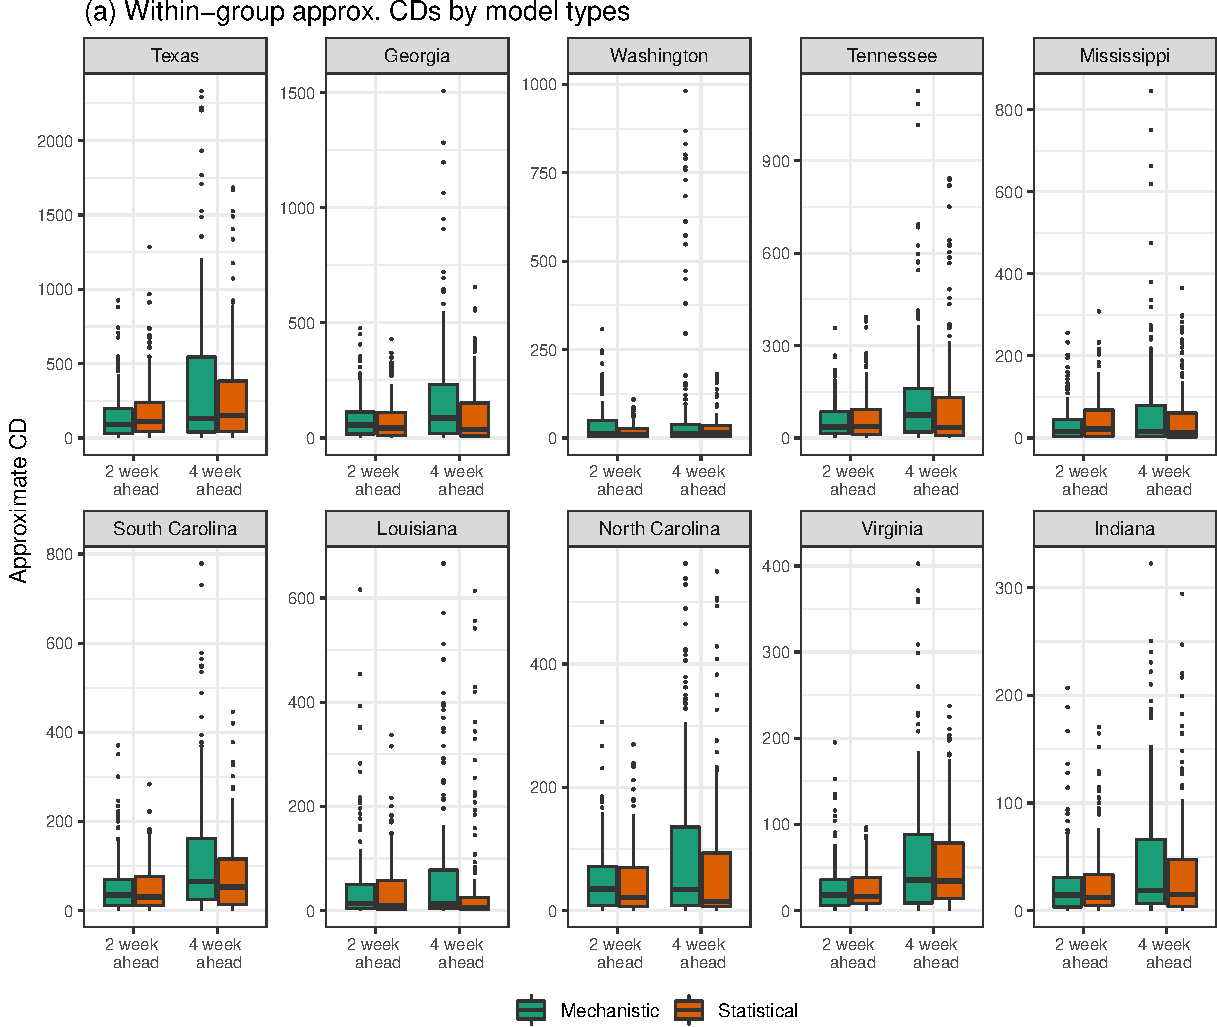
\includegraphics[width=1\linewidth,height=1\textheight]{multi_perm_analysis_files/figure-latex/box1-1} \end{center}

\begin{center}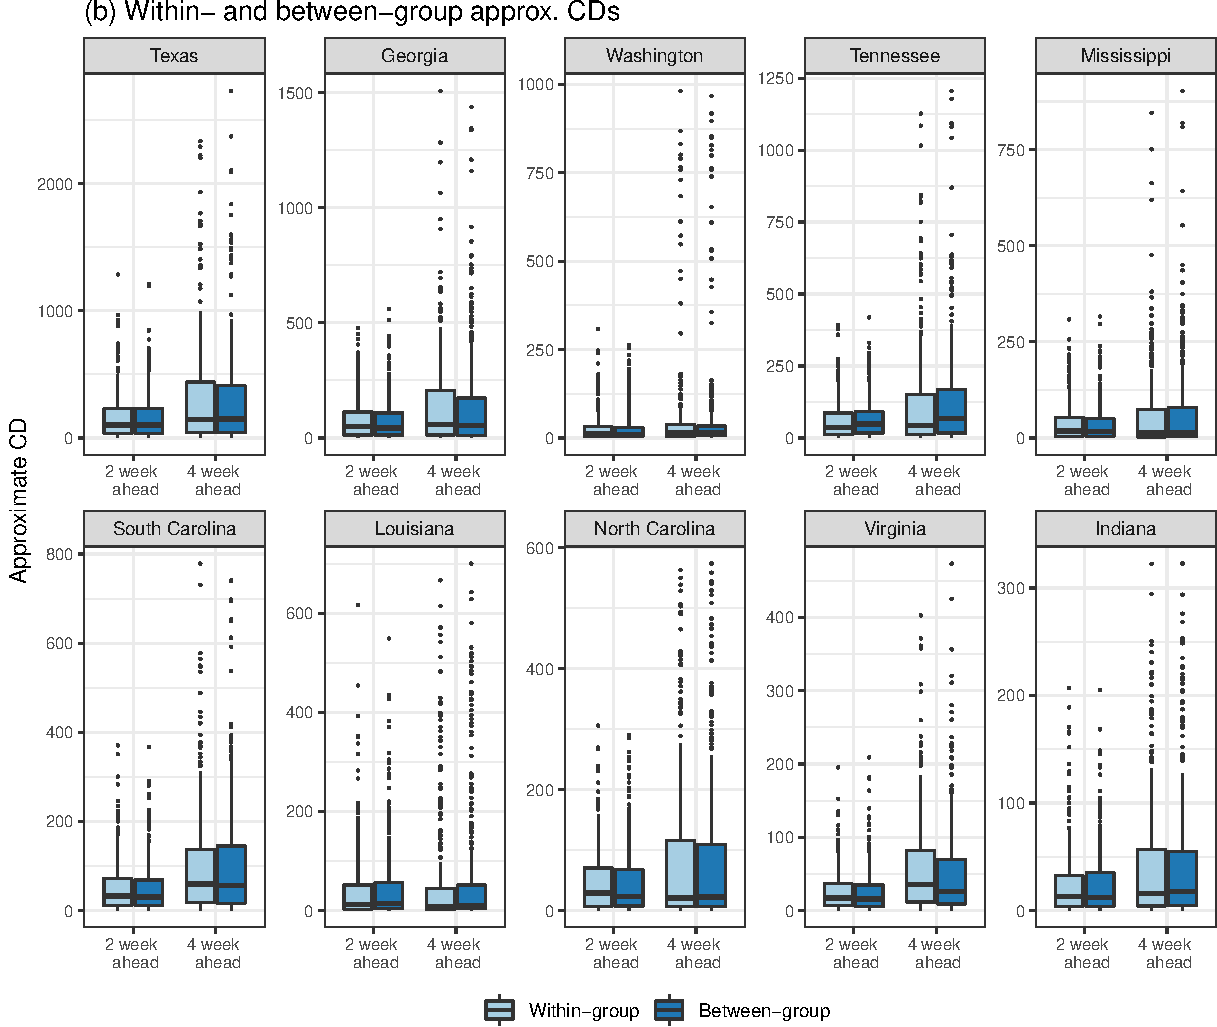
\includegraphics[width=1\linewidth,height=0.9\textheight]{multi_perm_analysis_files/figure-latex/box2-1} \end{center}

\hypertarget{distribution-of-test-statistics}{%
\subsection{Distribution of Test
Statistics}\label{distribution-of-test-statistics}}

Now that dates are irrelevant, more emphasis on locations.

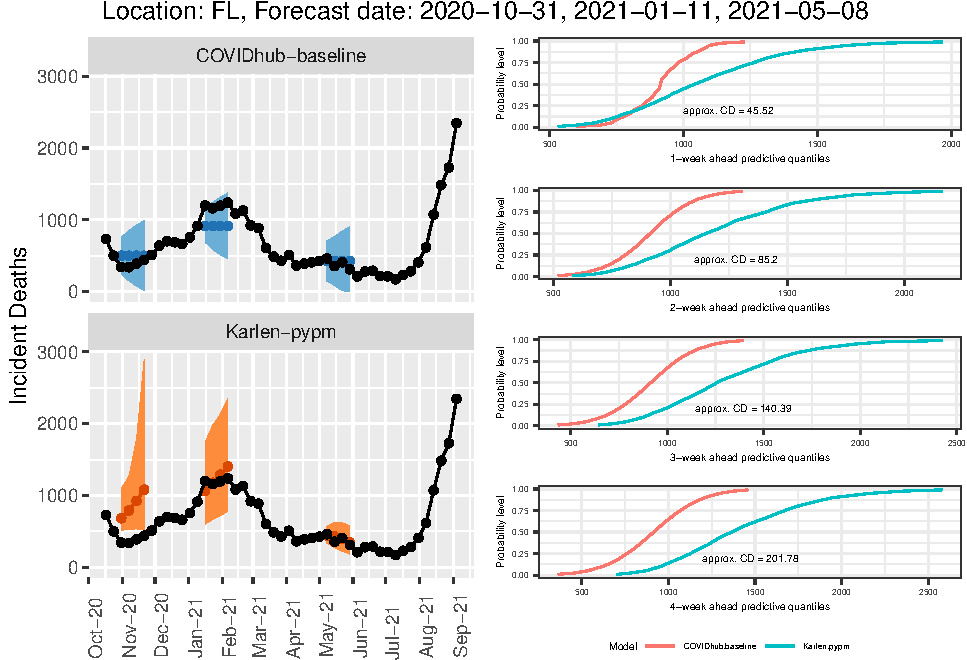
\includegraphics{multi_perm_analysis_files/figure-latex/unnamed-chunk-4-1.pdf}

\hypertarget{r-ggplotperm_statsl-geom_histogramaesxh2bins20filldarkgreen-geom_vlinexintercept-perm_statslh2_real1-annotatetext-label-paste0cexpressionrcdroundperm_statsh2_real12-x-1.12-y-320-size-4-colour-black-xlabtest-statistic-theme_bw-ggplotperm_statsl-geom_histogramaesxh4bins20filldarkgreen-geom_vlinexintercept-perm_statslh4_real1-annotatetext-label-paste0cexpressionrcdroundperm_statsh4_real12-x-1.18-y-320-size-4-colour-black-xlabtest-statistic-theme_bw}{%
\section{\texorpdfstring{\texttt{\{r\}\ \#\ ggplot(perm\_statsl)\ +\ \#\ \ \ geom\_histogram(aes(x=h2),bins=20,fill="darkgreen")\ +\ \#\ \ \ geom\_vline(xintercept\ =\ perm\_statsl\$h2\_real{[}1{]})+\ \#\ \ \ \#\ annotate("text",\ label\ =\ paste0(c(expression("R"{[}"CD"{]}),round(perm\_stats\$h2\_real{[}1{]},2))),\ \#\ \ \ \#\ \ \ \ \ \ \ \ \ \ x\ =\ 1.12,\ y\ =\ 320,\ size\ =\ 4,\ colour\ =\ "black")+\ \#\ \ \ xlab("Test\ statistic")+\ \#\ \ \ theme\_bw()\ \#\ ggplot(perm\_statsl)\ +\ \#\ \ \ geom\_histogram(aes(x=h4),bins=20,fill="darkgreen")\ +\ \#\ \ \ geom\_vline(xintercept\ =\ perm\_statsl\$h4\_real{[}1{]})+\ \#\ \ \ \#\ annotate("text",\ label\ =\ paste0(c(expression("R"{[}"CD"{]}),round(perm\_stats\$h4\_real{[}1{]},2))),\ \#\ \ \ \#\ \ \ \ \ \ \ \ \ \ x\ =\ 1.18,\ y\ =\ 320,\ size\ =\ 4,\ colour\ =\ "black")+\ \#\ \ \ xlab("Test\ statistic")+\ \#\ \ \ theme\_bw()\ \#}}{\{r\} \# ggplot(perm\_statsl) + \#   geom\_histogram(aes(x=h2),bins=20,fill="darkgreen") + \#   geom\_vline(xintercept = perm\_statsl\$h2\_real{[}1{]})+ \#   \# annotate("text", label = paste0(c(expression("R"{[}"CD"{]}),round(perm\_stats\$h2\_real{[}1{]},2))), \#   \#          x = 1.12, y = 320, size = 4, colour = "black")+ \#   xlab("Test statistic")+ \#   theme\_bw() \# ggplot(perm\_statsl) + \#   geom\_histogram(aes(x=h4),bins=20,fill="darkgreen") + \#   geom\_vline(xintercept = perm\_statsl\$h4\_real{[}1{]})+ \#   \# annotate("text", label = paste0(c(expression("R"{[}"CD"{]}),round(perm\_stats\$h4\_real{[}1{]},2))), \#   \#          x = 1.18, y = 320, size = 4, colour = "black")+ \#   xlab("Test statistic")+ \#   theme\_bw() \#}}\label{r-ggplotperm_statsl-geom_histogramaesxh2bins20filldarkgreen-geom_vlinexintercept-perm_statslh2_real1-annotatetext-label-paste0cexpressionrcdroundperm_statsh2_real12-x-1.12-y-320-size-4-colour-black-xlabtest-statistic-theme_bw-ggplotperm_statsl-geom_histogramaesxh4bins20filldarkgreen-geom_vlinexintercept-perm_statslh4_real1-annotatetext-label-paste0cexpressionrcdroundperm_statsh4_real12-x-1.18-y-320-size-4-colour-black-xlabtest-statistic-theme_bw}}

\begin{verbatim}
FALSE [1] "p-value for 2 wk horizon is 0.495337995337995"
\end{verbatim}

\begin{verbatim}
FALSE [1] "p-value for 4 wk horizon is 0.337412587412587"
\end{verbatim}

\end{document}
